\documentclass[conference]{IEEEtran}
\usepackage{graphicx}
\usepackage{cite}
\usepackage{url}
\usepackage[cmex10]{amsmath}
\usepackage{algorithmic}
\usepackage{array}
\usepackage{mdwmath}
\usepackage{mdwtab}
\usepackage{eqparbox}
\usepackage[font=footnotesize]{subfig}
\usepackage{fixltx2e}
\usepackage{setspace}
\usepackage{algorithm2e}
\usepackage{amssymb}



\begin{document}

\title{\large{CS388 NLP Project Report}\\ \huge{Text Mining for Hidden Relations and Trending}}

\author{\IEEEauthorblockN{C. Vic Hu}
\IEEEauthorblockA{vic@cvhu.org}
\and
\IEEEauthorblockN{Ali Unwala}
\IEEEauthorblockA{aliunwala@gmail.com}
}
\maketitle
\onehalfspace
\begin{abstract}
The main contributions of this paper are two fold. First, we formalize an illustration method to visualize topic trending on a spanning tree, which gives a meaningful intuition to discover how hidden thematic structures in large archive of text documents change, merge and split over time. Second, we propose a new algorithm, Thematic Particle Clustering, that combines probabilistic sampling, clustering and hill-climbing methods to predict upcoming topics based on a sequence of history topics. The effectiveness of our methods is demonstrated through a collection of 10,000 patents in the field of robotics spanning over 30 years.
\end{abstract}

%Motivate and abstractly describe the problem you are addressing and how you are addressing it. What is the problem? Why is it important? What is your basic approach? A short discussion of how it fits into related work in the area is also desirable. Summarize the basic results and conclusions that you will present. 
\section{Introduction}

Trending prediction and forecasting have been well-developed in stock market, economics, meteorology, physics and computer science. Most of the time we can formalize a probabilistic model to describe transitions from one state to another based on the observed history. However, such methods cannot be directly applied to text data for its lack of observables to be analyzed. Therefore, we need a more sophisticated way to make predictions for natural language.

In this paper, we developed a data visualization technique and a topic prediction algorithm. By parsing the US patents in the field of `robot' and `robotic', we obtained 10,000 text data spanning over 33 years, from 1981 all the way to 2013. These patents were sliced by each year and passed to Mallet \cite{mallet} for latent Dirichlet analysis \cite{lda2003} to obtain a collection of topic distributions. Our methods are then built on top of the results from the topic modeling algorithm.

To help observe the topic trending from year to year, we first developed a visualization technique to aid our analysis. Topics obtained from the text data intrinsically create twisted structures inherited from the previous years. To better understand the underlying patterns, we made a visualization technique, known as the Tree Convergence Graph (TCG). A TCG shows how topics split up, merge together, appear and disappear over a period of time. Our visualization technique superimposes topics from year to year until they converge, creating a bidirectional tree structure that is meaningful to read. We found this style of visualization novel and immensely useful in understanding topic relationships as they grew. 


Next, we proposed a topic prediction algorithm called Thematic Particle Clustering (TPC), which creates a collection of sampling particles, climb towards the closest topics and form cluster with others iteratively. We then used the clustering patterns to quantitatively describe how the future topics will be like. We made two assumptions that topics are conditionally dependent on previous topics, and that the topics modeling algorithm can be simulated with clustering methods. The efficacy of TPC was then demonstrated with the experimental results on the robotic patents dataset.
%The second contribution of this paper was a new topic modeling method called Thematic Particle Clustering (TPC). TPC treats each set of words in a topic as a vector. This vector is replicated into particles which are biased by the words counts for that year. We then choose the most relevant particles for a year and perform error analysis. The intuition for this idea is that we are more interested in the topics that have the highest word count for a year and these topics will have lower error from year to year.

In section 2, we give a brief background on the topic modeling algorithms, and specifically how Latent Dirichlet Analysis (LDA) works.  Section 3 describes the algorithms for TCG and TPC. Section 4 gives an example of TCG and carried out a rigorous evaluation of TPC. Section 5 and 6 includes the related works and how we can improve our current works, followed by a conclusion in section 7.

\section{Background}

Given a collection of text-based patent documents, one intuitive idea to find out trending patterns is to examine the underlying thematic structures hidden in the text. Based on the vocabulary distribution, we want to know what the intrinsic topics are implied in the given context. One common way to do exactly that is the Probabilistic Topic Models formalized by  Blei et al. \cite{blei2011}

\subsection{Probabilistic Topic Models}

The main objective of topic modeling is to automatically discover the unobserved hidden structures -- the topics, per-document topic distributions, and the per-document per-word topic assignments, while a collection of text documents is the only observable variables. 

\begin{figure}[h]
    \center    
	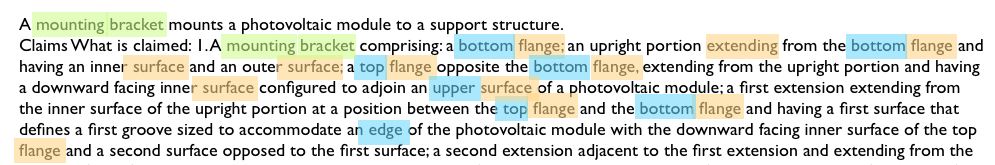
\includegraphics[width=0.45\textwidth]{fig/pat007.png}
	\caption{Text from a patent document}
	\label{sample_patent}
\end{figure}

For example in Fig.~\ref{sample_patent}, we have annotated a selection of words, with topics distinguished by colors. For the orange topic, we get words like flange, surface and extending, which could be interpreted as the attachment of hardware components. Similarly, the blue and green topics could be translated into topics about installation and mounting respectively. By looking at the text, human beings can infer what patent data in Fig.~\ref{sample_patent} is about, and accordingly highlight the relevant keywords that compose such topics. 

Nonetheless, the efficiency and accuracy of human labors does not scale when the size or complexity of these patent documents increases. The objective of probabilistic topic modeling is to automate this inference process and to provide hidden insights and meaningful intelligence to big data. If we are able to successfully construct a probable thematic structure from a large archive of text data for each time slice in a sequence, we could presumably infer how these topics inherit or inspire each other, and most excitingly, predict the most likely topics in the future.




\subsection{Latent Dirichlet Allocation}
Latent Dirichlet allocation, or LDA, is the simplest topic model \cite{lda2003} that assigns each word in the documents a distribution over a fixed number of topics. Instead of having a hard boundary between topic collections, LDA provides a distribution of topics per document, giving the likelihood of a mixed proportion of topic assignments. Namely, all text documents share the same set of topic collection but with different proportions to each topic. For instance in Fig.~\ref{topic_proportion}, although there are $K=100$ topics overall, only a few topics were actually activated in this particular patent.

\begin{figure}[h]
	\center
	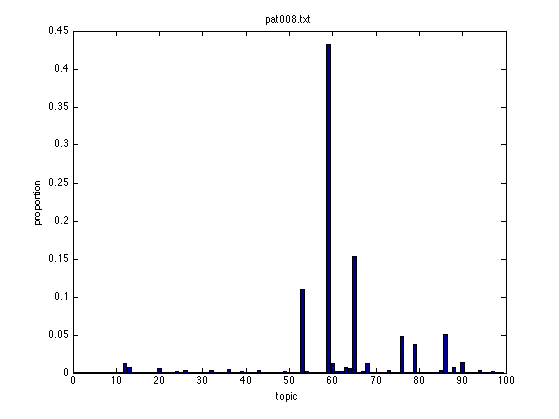
\includegraphics[width=0.25\textwidth]{fig/pat8_topics.png}
	\caption{A sample topic proportion of a patent}
	\label{topic_proportion}
\end{figure}




\begin{table}[h]
	\center
	\begin{tabular}{l p{5.5cm}}
$\beta_k,\; k = 1 \cdots K$& The K topics, represented by a distribution over words.\\
$\theta_d,\; d = 1 \cdots D$& Topic proportions for document d, where $\theta_{d,k}$ is the topic proportion of topic k for document d.\\
$z_d,\; d = 1 \cdots D$& Topic assignments for document d, where $z_{d,n}$ is the topic assignment for the n-th word in document d.\\
$w_d,\; d = 1 \cdots D$& The observed words for document d, where $w_{d,n}$ is the n-th word in document d.\\
	\end{tabular}
	\caption{Topic modeling notations}
	\label{tm_notations}
\end{table}
	
%
%\begin{description}
%	\item [$\beta_k,\; k = 1 \cdots K$]: the K topics, represented by a distribution over words
%	\item [$\theta_d,\; d = 1 \cdots D$]: topic proportions for document d, where $\theta_{d,k}$ is the topic proportion of topic k for document d
%	\item [$z_d,\; d = 1 \cdots D$]: topic assignments for document d, where $z_{d,n}$ is the topic assignment for the n-th word in document d
%	\item [$w_d,\; d = 1 \cdots D$]: observed words for document d, where $w_{d,n}$ is the n-th word in document d
%\end{description}
To build the generative probabilistic model, we compute the joint distribution and use it to estimate the posterior probability. With the notation specified in Table~\ref{tm_notations}, the LDA generative process can be formalized as the following joint probability of both hidden and observed random variables:

\begin{align*}
	&p(\beta_{1:K}, \theta_{1:D}, z_{1:D}, w_{1:D})\\
	=& \prod_{i=1}^K p(\beta_i)\prod_{d=1}^D p(\theta_d) \left( \prod_{n=1}^N p(z_{d,n} | \theta_d) p(w_{d,n} | \beta_{1:K}, z_{d,n})\right)
\end{align*}

Which can also be expressed graphically as:
\begin{figure}[h]
	\center
	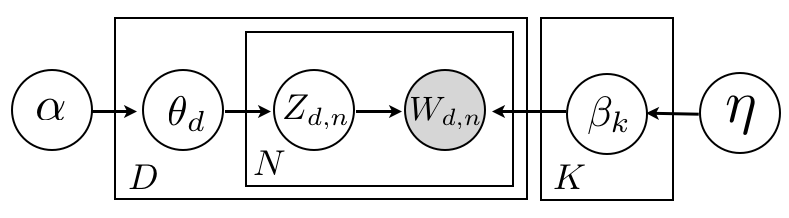
\includegraphics[width=0.35\textwidth]{fig/gm.png}
	\caption{LDA graphical model. Nodes represent variables, while edges indicate the dependency relations. The shaded node is the only observed variable (document words), and all others are the hidden variables. The $D$ plate denotes the replicated variables product over $D$ documents, while the $N$ plate denotes replication over $N$ words in each document.}
	\label{graphical_model}
\end{figure}

It is important to note that there are several conditional dependencies implied in the graphical models, which reflects the main principles of how LDA assumes the documents are generated:

\begin{enumerate}
\item Randomly pick a distribution $\theta_d$ over topics.
\item For each word in the document
	\begin{enumerate}
	\item Randomly choose a topic from the previously-chosen distribution $\theta_{d,n}$.
	\item Randomly choose a word from the corresponding distribution $Z_{d,n}$.
	\end{enumerate}
\end{enumerate}

Assuming this generative process is how our documents are created, now LDA uses the graphical model in Fig.~\ref{graphical_model} to infer the posterior probability of the hidden structures given our observable:

\begin{equation*}
p(\beta_{1:K}, \theta_{1:D}, z_{1:D} | w_{1:D}) = \frac{p(\beta_{1:K}, \theta_{1:D}, z_{1:D}, w_{1:D})}{p(w_{1:D})}
\end{equation*}

The computation of possible topic structures is often intractable and the posterior distribution can only be approximated in most cases. To form an approximation algorithm, topic modeling can generally be categorized as sampling-based algorithms and variational algorithms. The most popular sampling method for topic modeling is Gibbs sampling, which introduces a sequence of random variables to construct a Markov chain and collects samples from the limiting distribution to estimate the posterior. Instead of using samples to approximate the posterior, variational methods find the closest parameterized distribution candidate by solving optimization problems \cite{lda2003} \cite{bach2010}.

\begin{figure}[h]
	\center
	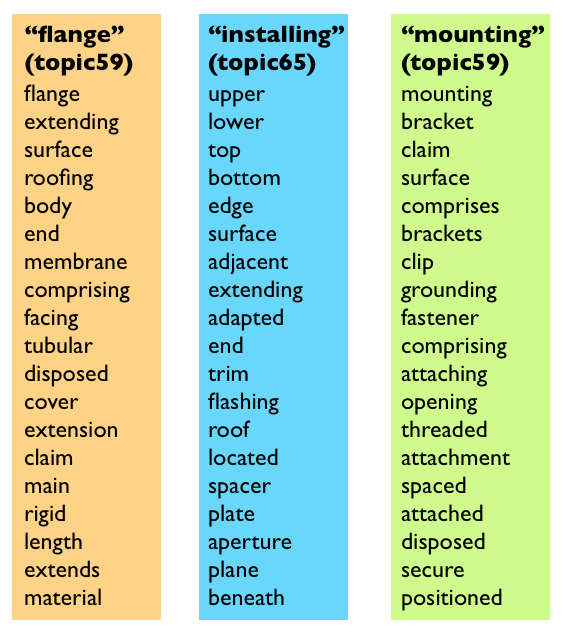
\includegraphics[width=0.25\textwidth]{fig/topics.png}
	\caption{The top 3 topics of a sample patent}
	\label{top3topics}
\end{figure}





\subsection{Limitations \& Potential Improvements}
Although LDA provides a powerful perspective to browsing and interpreting the implicit topic structures in our patent corpus, there are limitations it imposes against further discoveries. An extensive amount of research has been focused on relaxing some of the assumptions made by LDA to make it more flexible and suitable for more sophisticated information retrieval. 

LDA is essentially a bag-of-words probabilistic model. Namely, it constructs a word-frequency vector for each document but disregards the word ordering and the neighboring context. Although this assumption looses the syntactic information and sometimes seems unrealistic when processing natural language, it is usually good enough when capturing the document semantics and simplifying hidden structural inferences. Nonetheless, for more sophisticated tasks such as language generation or writing style modeling, the bag-of-words assumption is insufficient and needs to be relaxed. In these cases, there are variants of topic models that generate topic words conditioned on the previous word \cite{wallach2006}, or switches between LDA and hidden Markov models (HMM) \cite{griffiths2005}.

The LDA graphical model in Fig.~\ref{graphical_model} is invariant to the ordering of our patent documents. Which is an inappropriate assumption if the hidden thematic structure is actually dependent on sequential information such as years published, which is typically seen in document collections spanning years, decades or centuries. To discover how the topics change over time, the dynamic topic model \cite{blei2006} treats topics as a sequence of distributions over words and tracks how they change over time.

In either LDA or more sophisticated dynamic topic models \cite{blei2006}, the number of topics $\beta_{1:K}$ is determined manually and assumed to be fixed. One elegant approach provided by the Bayesian non-parametric topic model \cite{teh2006} is to find a hierarchical tree of topics, in which new documents can now imply previously undiscovered topics.

To include additional attribute information associated with the documents such as authorships, titles, geolocation, citations and many others, an active branch of research has been performed to incorporate meta-data in topic models. The author-topic model \cite{rosen-zvi2004} associates author similarity based on their topic proportions, the relational topic model \cite{blei2010} assumes document links are dependent on their topic proportion distances, and more general purpose methods such as Dirichlet-multinomial regression models \cite{mimno2008} and supervised topic models \cite{blei2007}.

Many other extensions of LDA are available, including the correlated topic model \cite{blei2007a}, pachinko allocation machine,  \cite{li2006}, spherical topic model \cite{reisinger2010}, sparse topic models \cite{wang2009} and bursty topic models \cite{doyle2009}.



\section{Problem Definition and Algorithm}
%Precisely define the problem you are addressing (i.e. formally specify the inputs and outputs). Elaborate on why this is an interesting and important problem. 


\subsection{Task Definition}

The primary objective of this paper is to learn from a given set of text documents and try to predict the upcoming themes. In particular, we focused on the US patents in the query results of `robot' and `robotic', consisting of over 10,000 documents from 1981 to 2013. To formalize the idea of how the thematic structures change in a sequence of text data, we applied LDA\cite{lda2003}, the simplest Topic Modeling we introduced in the previous section, to each time slices and found a collection of topics for each year. As mentioned previously, each topic is essentially a distribution over a set of words, which can be represented as a weighted vocabulary vector $\beta_i^y$ for the i-th topic in year $y$. Now we have a collection of topic vectors over a sequence of time, $\beta_{1:K}^{1:Y}$, our goal is to use this information to estimate the most likely topic vectors in the upcoming year, $\beta_{1:K}^{Y+1}$, from which we can interpret a reasonable prediction and quantitatively evaluate our performance.

%The primary task we are trying to solve with TPC is minimizing the error over years by making a modified topic using all our past knowledge. The idea here is if we are making a vector that is mimizing errors from year to year we are effectively predicting the future topic just by guessing a topic with a lower error.

%Describe in reasonable detail the algorithm you are using to address this problem. A psuedocode description of the algorithm you are using is frequently useful. Trace through a concrete example, showing how your algorithm processes this example. The example should be complex enough to illustrate all of the important aspects of the problem but simple enough to be easily understood. If possible, an intuitively meaningful example is better than one with meaningless symbols. 



\subsection{Tree Convergence Graph Algorithm}
Before we were able to parse the topic models we needed to be able to understand the data we were looking at. Our TCG algorithm followed the following steps 


\begin{verbatim}
1      Initialize array named PATHS
2      foreach YEAR:
3      |    foreach TOPIC:
4      |    |    PATHS = return path from  
       |    |    current node to the end 
       |    |    of years
5      |    end 
6      end 
7     
8      foreach PATH in PATHS:  
9      |    PATH = merge PATH with
10     |    other other PATHS 
11     end foreach path in paths
12    
13     plot(paths)
\end{verbatim}   

\subsection{Thematic Particle Clustering Algorithm}

Built on top the results obtained from the LDA topic models, our Thematic Particle Clustering (TPC) algorithm aims to make topic predictions for the upcoming year based on what the algorithm had seen in the past. Our goal is to formalize a set of particles $\mathbf{w}_{1:N}$ inferred from the topics from previous years, cluster them and use the results to describe what we The TPC al the upcoming topics $\mathbf{\beta}_{1:K}$ will be. Before jumping into the details of TPC, let's go over some of the fundamental concepts and definitions we will use.

\subsubsection{Distance Functions}
The idea of a particle is essentially a sampled instance of the topic distribution over a time sequence, represented by a vector $\mathbf{w}_i\in \mathbb{R}^{|V|},\; i \in \{1,\cdots,N\}$, where $|V|$ is the total vocabulary size of all the topic words appeared. Since one of our intermediate objectives is to formalize clusters between these particles, we need to first define how we will measure the similarity or distance between any pair of particles $\mathbf{w}_i,\; \mathbf{w}_j$. 

\-\\
\textbf{Minkowski}: 
\begin{equation*}
	d = \sqrt[p]{\sum_{k=1}^{|V|}|w_{ik} - w_{jk}|^p}
\end{equation*}
 Note that when $p=1$, the Minkowski reduces to the city block distance, while $p=2$ gives the Euclidean distance and $p=\infty$ yields the Chebychev distance.

\-\\
\textbf{Cosine}: 
\begin{equation*}
d = 1 - \frac{\mathbf{w}_i\,\mathbf{w}_j^T}{|\mathbf{w}_i|_2|\mathbf{w}_j|_2}
\end{equation*}

\-\\
\textbf{Correlation}: 
\begin{equation*}
d = 1 - \frac{(\mathbf{w}_i - \overline{\mathbf{w}}_i)(\mathbf{w}_j - \overline{\mathbf{w}}_j)^T}{|(\mathbf{w}_i - \overline{\mathbf{w}}_i)|_2|(\mathbf{w}_j - \overline{\mathbf{w}}_j)|_2}
\end{equation*}

where 
\begin{equation*}
	\overline{\mathbf{w}}_i = \frac{1}{|V|}\sum_{k=1}^{|V|}w_{ik},\;
	\overline{\mathbf{w}}_j = \frac{1}{|V|}\sum_{k=1}^{|V|}w_{jk}
\end{equation*}

\-\\
\textbf{Jaccard}: 
\begin{equation*}
	d = \frac{\# \left[(w_{ik} \neq w_{jk})\cap((w_{ik} \neq 0)\cup(w_{jk} \neq 0))\right]}{\#\left[(w_{ik} \neq 0)\cup(w_{jk} \neq 0)\right]}
\end{equation*}

\-\\

\subsubsection{Clustering Algorithms}
LDA is essentially pulling out the `principal components' from the text documents, reducing a large archive of data into just $K$ representative topics $\mathbf{\beta}_{1:K}$. Therefore, our assumption is that by grouping similar particles induced from past topics, we can observe the clustering patterns and make reasonable predictions on how the future topics will act.

Now we have a collection of well-defined distance functions, we can start looking at clustering methods to group our particles together accordingly, and here are a set of common clustering algorithms we consider:

\-\\
\textbf{K-Means:} As the name itself suggests, the K-Means clustering algorithm consists of K cluster centroids and moves these means iteratively towards the center of its closest neighbors, until they no longer change. Although K-Means has been proved to be guaranteed for convergence \cite{selim1984}, its clustering performance is often correlated to how the seeds are initialized, and the optimal choice of $K$ is often not apparent (in our case, $K$ is the same as the number of topics.)

\begin{verbatim}
1. Initialize the means by picking 
   K samples at random
2. Iterate
2.a. Assign each instance to 
     its nearest mean
2.b. Move the current means to 
	 the center of all the 
	 associated points
\end{verbatim}
\-\\
\textbf{Hierarchical Agglomerative Clustering (HAC):} This algorithm starts with treating every instances as individual cluster, and iteratively joins pairs of similar clusters repeatedly until there is only one. If we take the merging history and form a hierarchical binary tree, it will look like the dendrogram in Fig.~\ref{dendrogram}.

\begin{figure}[h]
	\center	
	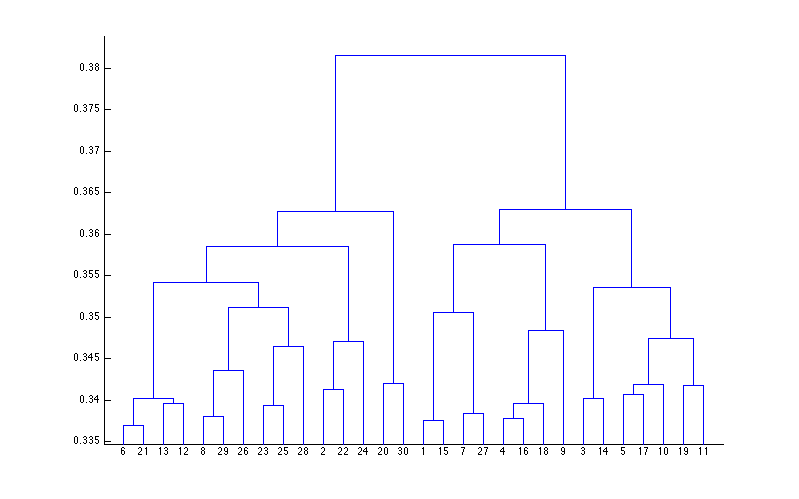
\includegraphics[width=0.35\textwidth]{fig/dendrogram.png}
	\caption{A sample dendrogram by HAC}
	\label{dendrogram}
\end{figure}

Although we have defined the distance functions in the previous section, we have yet formalized the similarity functions between clusters. In our method, we will focus on the following four similarity functions:

\begin{itemize}
	\item \textbf{Single-linkage:} Also known as the nearest neighbor, computes the distance between the two closest elements from two clusters
	\item \textbf{Complete-linkage:} The conjugate of \textbf{single-linkage}, also known as the farthest neighbor, computes the distance between the two farthest elements (maximum distance) from two clusters
	\item \textbf{UPGMA: } Unweighted Pair Group Method with Averaging calculates the distance between two clusters, $C_i \& C_j$, by averaging all distances between any pair of objects from the two clusters.
	\begin{equation*}
		dist(C_i, C_j) = \frac{1}{|C_i||C_j|}\sum_{w_i \in C_i}\sum_{w_j \in C_j}dist(w_i, w_j)
	\end{equation*}
	Now, let's call this newly-formed cluster $C_{ij}$ and compare its distance with another cluster $C_k$:
	\begin{equation*}
		dist(C_{ij}, C_k) =  \frac{|C_i|dist(c_i,c_k) + |C_j|dist(c_j,c_k)}{|C_i|+|C_j|}
	\end{equation*}
	where $c_i,\,c_j,\,c_k$ are the centroids for clusters $C_i,\;C_j,\;C_k$
	\item \textbf{WPGMA} Weighted Pair Group Method with Averaging is similar to UPGMA except that the cluster distance is now calculated as:
	\begin{equation*}
		dist(C_{ij}, C_k) =  \frac{dist(c_i,c_k) + dist(c_j,c_k)}{2}
	\end{equation*}
\end{itemize}

 The behavior of HAC is often dominated by the chosen similarity function. While each variant has a different set of clustering patterns it is good at capturing, all of them have trade offs. 

\subsubsection{Putting It Altogether}

Now we have gone through all the necessary concepts we used, the concepts of our Thematic Particle Clustering (TPC) algorithm is pretty straightforward, which can be found in Table.~\ref{TPC_algorithm}. 

To simulate how the topic flow splits and merges over time, we introduce the concept of \emph{particles}. One key assumption we made here is that when the topics carry over to the next year, each topic from the current year actually splits up itself and redistribute its sub-components to merge with those from other topics. Namely, if we focus on just one topic at a time slice snapshot and see how it `flows' subsequently, what we get is a tree-like structure that describes how such topic splits up and merge together with other things to form future topics, or simply vanishes gradually. If we take all these tree-like structures from every topics and study how they behave over the years, what we end up with is a complex directional acyclic graph (DAG) similar to our city water system (see Fig.~\ref{tcg})

If we see this complex DAG, or what we call the Topic Convergence Graph (TCG), as a water system, the idea of the particles can be thought of as a school of clean sponge fishes released from the very upper division of the rivers. As these sponge fishes swim downstream, they start collecting flavors and colors along the path chosen. At the lower division, we can randomly sample a sponge fish, and extract some information about its traveled trajectory by observing its color and flavor combination. By injecting the sampling particles to flow with the topics, we hope to observe an accumulated momentum that will presumably help us predict its behavior in the future.

The above are the intuitions behind the Thematic Particle Clustering algorithm. We start by initializing a collection of particles uniformly assigned to each topic in the first year, with gaussian noise added to include stochasticity (controlled by a parameter $\alpha$.) For each time step (sliced by year), we apply the clustering algorithms mentioned above to group similar particles together, in which we made another assumption that LDA could be simulated by clustering similar particles. Once forming the $K$ clusters, we look at the topics from the next year and pick one that is the closest to each cluster. Finally, we do a hill-climb for all the particles within each cluster towards the corresponding optimal topic with a discount rate $\gamma$ to anneal old weights and the same gaussian noise controlled by $\alpha$ (see Step 5 in Table.~\ref{TPC_algorithm}), and repeat the same process for the next time step.

\begin{table}[h]
	\centering
	\begin{tabular}{r|p{7.25cm}}
		Step & Action\\
		\hline
		\hline
		1 & Initialize $\mathbf{w}_{1:N}=\beta^1_i + \mathbf{N}(0,\sigma(\beta^1_i))$ \\
		 & // Randomly assign each particle the i-th topic from the first year $\beta^1_i$\\
		 \hline
		2 & For $y = 2 \cdots (yo - 1)$\\
		 & // Iterate the following steps through each of the following years in the time sequence until reaching right before the predicting year $yo$\\
		 \hline
		3 & $\mathbf{c}=cluster(\mathbf{w}_{1:N}, K, dist, link)$\\
		& // Get the cluster index $\mathbf{c}$ from the clustering algorithm with the designated distance function $dist$ and the linkage $link$\\
		\hline
		4 & For $k = 1 \cdots K$ \\
		\hline
		5 & $\mathbf{w}_k = \gamma \, \mathbf{w}_k + \beta^y_j + \alpha\mathbf{N}(0,\sigma(\beta^y_j))$\\
		& // Iterate through each of the $K$ clusters to find the closest topics from the current year $\beta^y_j$, where $\mathbf{w}_k$ is defined as the particles assigned to cluster $k$. Apply $\gamma$, the discount rate, to the old weights and shift the new weights toward $\beta^y_j$ with an $\alpha$-strong gaussian noise\\
		\hline
		6 & End the for loops for both Step 2 and 4\\
	\end{tabular}
	\caption{The TPC Algorithm}
	\label{TPC_algorithm}
\end{table}

%\begin{verbatim}
%1. Initialize N particles
%2. Iterate
%2.a. Add Gaussian noise to particles
%2.b. Cluster particles into K groups
%2.b.1 If we are predicting the next year:
%	    Stop and return the clusters
%2.b.2 Else:
%        Compare the cluster centroids with 
%        topics from the next year, apply discounts to current weights, and adjust to new weights
%2.d. Repeat
%\end{verbatim}

\section{Experimental Evaluation}
%What are criteria you are using to evaluate your method? What specific hypotheses does your experiment test? Describe the experimental methodology that you used. What are the dependent and independent variables? What is the training/test data that was used, and why is it realistic or interesting? Exactly what performance data did you collect and how are you presenting and analyzing it? Comparisons to competing methods that address the same problem are particularly useful. 


\subsection{Methodology}
%Present the quantitative results of your experiments. Graphical data presentation such as graphs and histograms are frequently better than tables. What are the basic differences revealed in the data. Are they statistically significant? 

Before starting, we preprocessed the results obtained from LDA and constructed each topic in each year as vectors in the space of the entire vocabulary $\beta_{1:K}^{1:Y}$, as shown in Fig.~\ref{spy}. We can clearly observe the patterns of how the vocabulary evolved over the years, including repeated occurrence of certain words and the frontier curve that indicates newly-emerged word, which is also represented in Fig.~\ref{vocabs}.
\begin{figure}[h]
    \center    
	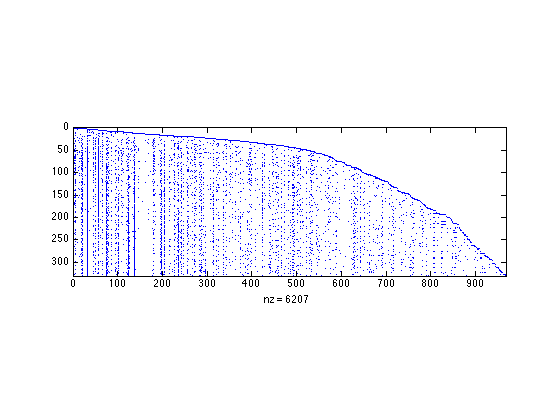
\includegraphics[width=0.45\textwidth]{fig/spy.png}
	\caption{A scatter plot showing patterns of the topics words over the years. The y-axis corresponds to the year-topics (10 topic/year X 33 years), while the x-axis show the 967 words appeared in the topic distributions.}
	\label{spy}
\end{figure}

\begin{figure}[h]
    \center    
	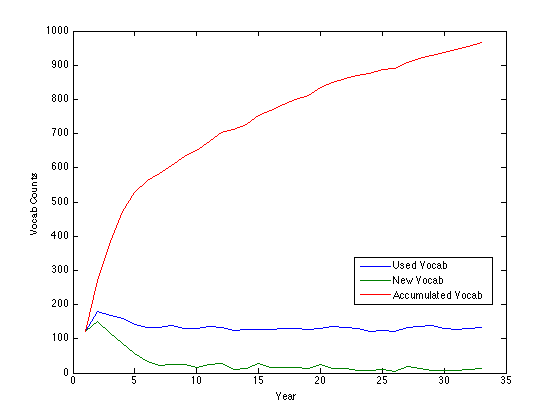
\includegraphics[width=0.35\textwidth]{fig/vocabs.png}
	\caption{A graph to show how new vocabularies are introduced over the years.}
	\label{vocabs}
\end{figure}


\subsubsection{Tree Convergence Graph}
The TCG was created out of necessity to gain intuition about the underlying data structure. TCG helped us formalize our ideas which led to the TPC method. TCG very quickly shows when large groups of topics appear. This structure gave us the intuition that topics could be word biased. Since topics with the most popular words for an year may be more important over time than just an random topics. TCG helped us gain an intuition for evaluating the TPC method by comparing how well a word biased error does with respect to an unbiased error.

\subsubsection{Thematic Particle Clustering}
We were successfully able to implement TPC. TPC was implemented twice with two clustering algorithms HAC and K-Means. We performed rigorous testing against various parameter values and with respect to different clustering algorithms and distance functions described in section 3.

Our TPC using HAC (TPC-HAC) evaluation has 4 components. First, we tested $\gamma$, the discount rate parameter, to see how annealing the weights from older years influences the learning performance. Second, we tested TPC-HAC while varying the noise factor, $\alpha$, which allowed us to study effects of adding stochasticity in $\mathbf{w}$ vectors. Third, we compared our clustering algorithms with a collection of distance functions. Finally, we looked at how the linkage functions in HAC affect our results.

Our evaluation of TPC using K-Means (TPC-KM) had 3 components. All of which were in a similar style to the TPC-HAC evaluation, except for the linkage function comparison, which only applies to HAC methods.

\subsection{Results}
%Is your hypothesis supported? What conclusions do the results support about the strengths and weaknesses of your method compared to other methods? How can the results be explained in terms of the underlying properties of the algorithm and/or the data. 

\subsubsection{Tree Convergence Graph}
For readability, we  present an example of a TCG in the Appendix A. On the X axis we show 10 years of patents and on the Y axis we have 10 topics per year. Each line on the graph shows the most probable link between a set of patents between 2 years. It is important to notice the ``dangling lines" that start midway though the graph (for example the green line at the bottom in 1985). These ``dangling lines" represent new topics appearing. It is also important to note that once a group of topics have converged to an single topic they will never again diverge. 

Appendix A shows only 10 of the 31 years of data we pulled from 1982 to 1991. We let the graph continue without adding adding any new ``dangling lines" and  by 1998 you can see every topic from between 1982-1991 has converged to just two separate topics. Each time a line changes color in Fig. \ref{tcg} this represents a new topic usurping an older one.

We make the assumption that every year a topic must go to a topic the next year. We believe this is a reasonable assumption for patents since inventions build on each other and would rarely skip a whole year before something new came out.

\subsubsection{Thematic Particle Clustering}

First, we compared TPC-HAC with various $\gamma$ values to see the effect of discount rate. In Fig.~\ref{hac_gamma} we have a baseline method that simply models each year's topics using only the ones from the previous year. We can immediately observe some improvements imposed by $\gamma=0.75,\;0.5$, and inferior performance led by $\gamma=1.0,\;0.0$ for no discount or learning at all. For the following experiments, we hold $\gamma=0.75$ as our optimal discount rate.

\begin{figure}[h]
	\center
	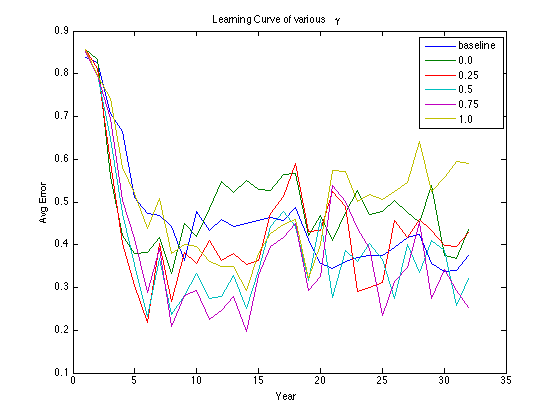
\includegraphics[width=.50\textwidth]{fig/hac_gamma.png}
	\caption{HAC Learning curve versus $\gamma$}
	\label{hac_gamma}
\end{figure}

Next, we compared the TPC-HAC learning curves against various stochasticity by tuning $\alpha$. In Fig.~\ref{hac_alpha}, it is shown that reduced stochasticity with smaller $\alpha$ actually yields better results, while varying $\alpha$ doesn't reshape the learning curve as dramatically as changing $\gamma$ in Fig.~\ref{hac_gamma}.

\begin{figure}[h]
	\center
	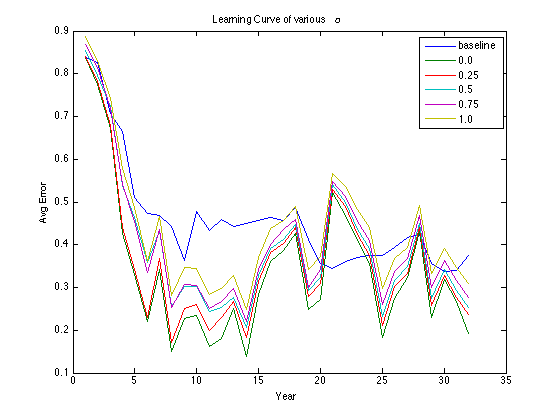
\includegraphics[width=.50\textwidth]{fig/hac_alpha.png}
	\caption{HAC Learning curve versus $\alpha$}
	\label{hac_alpha}
\end{figure}

To understand how the learning performance is dominated by the choice of distance functions, we compared the TPC-HAC learning curves using various distance functions covered in section 3 side-by-side. As shown in Fig.~\ref{hac_dist}, very little differences could be observed, which assured our assumption that the distance function doesn't impose much bias against TPC-HAC.

\begin{figure}[h]
	\center
	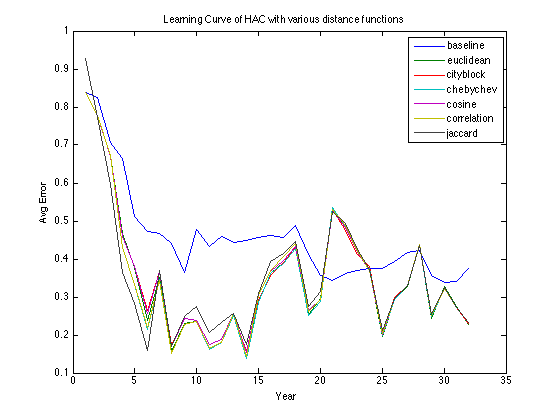
\includegraphics[width=.50\textwidth]{fig/hac_dist.png}
	\caption{HAC Learning curve versus distance function}
	\label{hac_dist}
\end{figure}

We did another similar test with different linkage functions in HAC and observed even less variation, as shown in Fig.~\ref{hac_link}. This result implies uniform and convex shaping of how the particles are distributed in the vocabulary vector space.

\begin{figure}[h]
	\center
	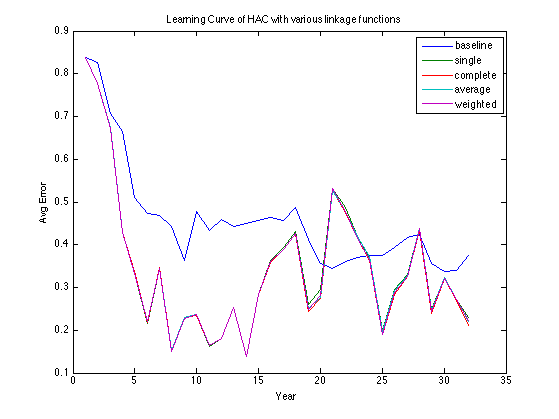
\includegraphics[width=.50\textwidth]{fig/hac_link.png}
	\caption{HAC Learning curve versus linkage function}
	\label{hac_link}
\end{figure}

These experiments show conclusively that TPC-HAC has a promising potential in topic prediction, and that the idea of using particle to sample, cluster and hill-climb towards the optimal topic is a reasonable approach.

Now we look at our second implementation of TPC using the K-means clustering algorithm, TPC-KM. We again started by testing $\gamma$. From Fig.~\ref{kmeans_gamma}, we can see a similar optimal $\gamma$ as in TPC-HAC, with little shared patterns.

\begin{figure}[h]
	\center
	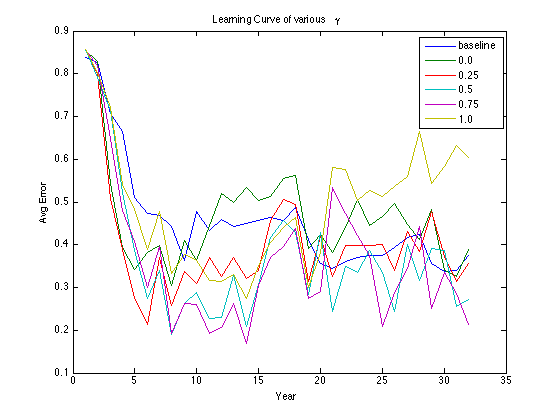
\includegraphics[width=.50\textwidth]{fig/kmeans_gamma.png}
	\caption{K-Means Learning curve versus $\gamma$}
	\label{kmeans_gamma}
\end{figure}

Fig.~\ref{kmeans_alpha} also yields a very similar pattern of learning curves as we study it's relationships with $\alpha$; we got a slightly smaller error rate with less stochasticity.
%
%The second test for TPC-KM looks for the optimal $\alpha$. Here we get an different optimal result, looking at Fig. \ref{kmeans_alpha} we see that an 0.25 $\alpha$ looks optimal.

\begin{figure}[h]
	\center
	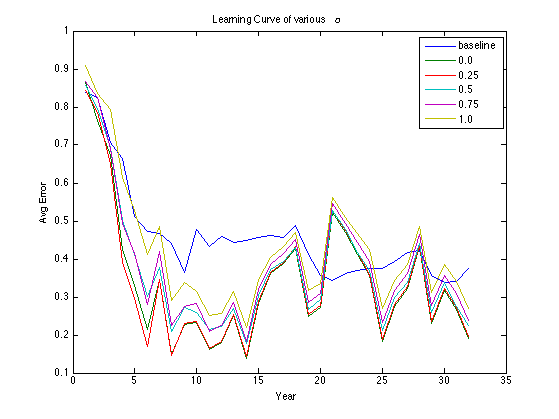
\includegraphics[width=.50\textwidth]{fig/kmeans_alpha.png}
	\caption{K-Means Learning curve versus $\alpha$}
	\label{kmeans_alpha}
\end{figure}

Finally, we tested how different distance functions influence the behavior in the phase of the K-means clustering. By looking at Fig.~\ref{kmeans_dist}, we again observed little differences between distant functions, except for ``city block'', which is the same as the $L_1$ norm.
\begin{figure}[h]
	\center
	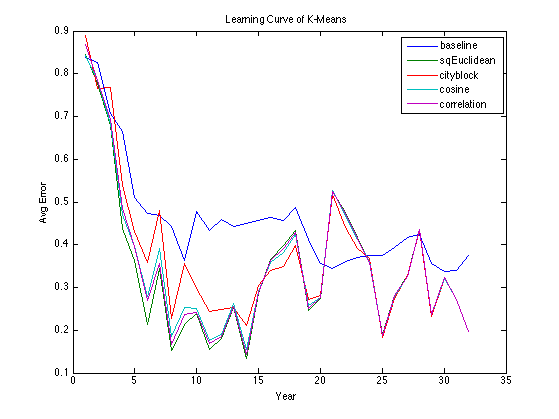
\includegraphics[width=.50\textwidth]{fig/kmeans_dist.png}
	\caption{K-Means Learning curve versus distance function}
	\label{kmeans_dist}
\end{figure}


Both TPC-HAC and TPC-KM constantly outperformed the baseline method in almost every year in our patent data, with an average improvement of 11\% and 12\% respectively over 33 years.

\subsection{Discussion}

\subsubsection{Tree Convergence Graph}
TCGs are a great tool to visualize data but have trade offs. For example a TCG will not directly show you why two topics decided to merge. Nor does it tell you what words a topic is made up of. Or how strongly the topics converged. These issues could be added to the TCG graph but would make the data less parseable. Some other features like word counts for the entire year would just not make sense in the TCG graph. Regardless of some of these drawbacks we still believe visualizing this data provided an important starting point for building intuition about the data.

\subsubsection{Thematic Particle Clustering}
Based on our experimental results, the TPC algorithm has a promising potential in predicting topics obtained from LDA. They are both dependent on the choice of discount rate $\gamma$, with little bias introduced when choosing different noise level $\alpha$. Although both TPC-HAC and TPC-KM perform better than the baseline method in most years, the learning curve doesn't go down monotonically with more years of data, as one might expect. All of our results consistently have rising errors. In fact, TPC is even worse than the baseline methods between year 21 and 24. One way to explain this result is large amount of new topic additions in certain years, which couldn't be predicted using the topics from the past. Since our patent data was pulled from the robotic-related literature, it makes sense that we would see evolutionary innovations in the late 90s and after 2000. If we were to use TPC on a more established field, the performance may appears more reliable and promising, which remains as a subject for our future works.


%Answer the following questions for each piece of related work that addresses the same or a similar problem. What is their problem and method? How is your problem and method different? Why is your problem and method better? 

\section{Related Work}
Our method for choosing the most probable path of topics builds on the ideas of the Viterbi Algorithm (VA)\cite{viterbi}. Our predictions for topics are made by finding the error between topics from year to year. In any two given years our algorithm will find the lowest error for every topic from one year to the next. With this information we can build a forward trellis structure from every starting topic.

The dynamic topic models (DTM) developed by Blei et al. \cite{blei2006} builds a generative graphical model to study how the topics change over time, which could be very useful for trend prediction. However, DTM assumes a fixed set of topics throughout the entire time sequence, and it only samples how the proportions of the same set of topics change over time. Although we also assume that the number of topics is fixed over the years, our topic models were calculated by a conventional LDA individually for each year, which reflects a more direct perspective on the true topics formed by each time slice.

%What are the major shortcomings of your current method? For each shortcoming, propose additions or enhancements that would help overcome it. 
\section{Future Work}
Building on this work there are many paths that could lead additional research.

First, our implementation of TPC biases particles with respect to word counts. There could be better features to try and bias results by, for example authors or document length. Finding a better set of features to bias words by could be done by creating an large set of features for each document and seeing which set of features are most correlated from year to year. Correlations could be found through tools like Weka. 

Another way to modify TPC's could be through using multilayer neural network compression techniques on the particles. In the TPC algorithm $N>K$ where $N$ is the number of particles and K is the number of topics. We have to provide a transform to fit $N$ into $K$ so it can be used from year to year. Using a neural network with an appropriately defined error function we could transform $N$ particles into $K$ particles with multiple features weighting the distribution.

Finally, more sophisticated methods can be introduced when measuring the similarity between two topics. Techniques such as Kullback-Leibler divergence, information entropy gains and TF-IDF could be very useful directions to consider for future research and development. 

%Briefly summarize the important results and conclusions presented in the paper. What are the most important points illustrated by your work? How will your results improve future research and applications in the area? 
\section{Conclusion}

To study the hidden relations in a large archive of patent text data, we applied the topic modeling algorithm, LDA, to each time slice individually and built the Topic Convergence Graph to help us visualize topics trending and their inheritance relations. Furthermore, we introduced a topic prediction algorithm, Thematic Particle Clustering, which generates a number of sampling particles to capture information spillovers between years and uses their clustering patterns to forecast future topics. Compared with a baseline method, we were able to make a decent improvement of 11-12\% on average. Although there are many ways we can improve upon our method to provide a more reliable and accurate prediction, we believe our works opened a promising door for further research in the field and demonstrated the possibility of predicting topic trends in text data.


\section{Acknowledgement}

We are very grateful to the valuable feedback and suggestions given by Professor Mooney at the University of Texas at Austin. We would also like to thank Blei et al. for building up the ground works behind topic modeling, and McCallum et al. for the development of MALLET.

%Be sure to include a standard, well-formated, comprehensive bibliography with citations from the text referring to previously published papers in the scientific literature that you utilized or are related to your work.
\begin{thebibliography}{1}

\bibitem{blei2011}
Blei, D. Introduction to Probabilistic Topic Models. Princeton University. 2011.

\bibitem{lda2003}
Blei, D., Ng, A. and Jordan, M. Latent Dirichlet allocation. Journal of Machine Learning Research, 3:993-1022, January 2003.

\bibitem{bach2010}
Hoffman, M., Blei, D. and Bach, F. On-line learning for latent Dirichlet allocation. In Neural Information Processing Systems, 2010.

\bibitem{wallach2006}
Wallach, H. Topic modeling: Beyond bag of words. In Proceedings of the 23rd International Conference on Machine Learning, 2006.

\bibitem{griffiths2005}
Griffiths, T., Steyvers, M., Blei, D. and Tenenbaum, J. Integrating topics and syntax. In L. K. Saul, Y. Weiss, and L. Bottou, editors, Advances in Neural Information Processing Systems 17, pages 537-544, Cambridge, MA, 2005. MIT Press.

\bibitem{blei2006}
Blei, D. and Lafferty, J. Dynamic topic models. In International Conference on Machine Learning, pages 113-120, New York, NY, USA, 2006. ACM

\bibitem{teh2006}
Teh, Y., Jordan, M., Beal, M. and Blei, D. Hierarchical Dirichlet process. Journal of the American Statistical Association, 101(476):1566-1581, 2006.

\bibitem{rosen-zvi2004}
Rosen-Zvi, M., Griffiths, T., Steyvers, M. and Smith, P. The author-topic model for authors and documents. In Proceedings of the 20th Conference on Uncertainty in Artificial Intelligence, pages 487-494. AUAI Press, 2004.

\bibitem{blei2010}
Chang, J. and Blei, D. Hierarchical relational models for document networks. Annals of APplied Statistics, 4(1), 2010.

\bibitem{mimno2008}
Mimno, D. and McCallum, A. Topic models conditioned on arbitrary features with Dirichlet-multinomial regression. In Uncertainty in Artificial Intelligence, 2008.

\bibitem{blei2007}
Blei, D. and McAuliffe, J. Supervised topic models. In Neural Information Processing Systems, 2007.

\bibitem{blei2007a}
Blei, D. and Lafferty, J. A correlated topic model of Science. Annals of Applied Statistics, 1(1):17-35, 2007.

\bibitem{li2006}
Li, W. and McCallum, A. Pachinko allocation: DAG-structured mixture models of topic correlations. In International Conference on Machine Learning, pages 577-584, 2006.

\bibitem{reisinger2010}
Reisinger, J., Waters, A. ,Silverthorn, B. and Mooney, R. Spherical topic models. In International Conference on Machine Learning, 2010.

\bibitem{wang2009}
Wang, C. and Blei, D. Decoupling sparsity and smoothness in the discrete hierarchical dirichlet process. In Y. Bengio, D. Schuurmans, J. Lafferty, C. K. I. Williams, and A. Culotta, editors, Advances in Neural Information Processing Systems 22, pages 1982-1989. 2009.

\bibitem{doyle2009}
Doyle, G. and Elkan, C. Accounting for burstiness in topic models. In International Conference on Machine Learning, pages 281-288. ACM, 2009.

\bibitem{selim1984}
Selim, S. Z. and Ismail, M. A. (1984). K-means-type algorithms: a generalized convergence theorem and characterization of local optimality. Pattern Analysis and Machine Intelligence, IEEE Transactions on, (1), 81-87.


\bibitem{mallet}
McCallum, A. K. (2002). Mallet: A machine learning for language toolkit.

\bibitem{viterbi}
Forney Jr, G. D. (1973). The viterbi algorithm. Proceedings of the IEEE, 61(3), 268-278.

\end{thebibliography}

\section{Appendix}
\section{Appendix A}
\begin{figure*}[h]
	\center
	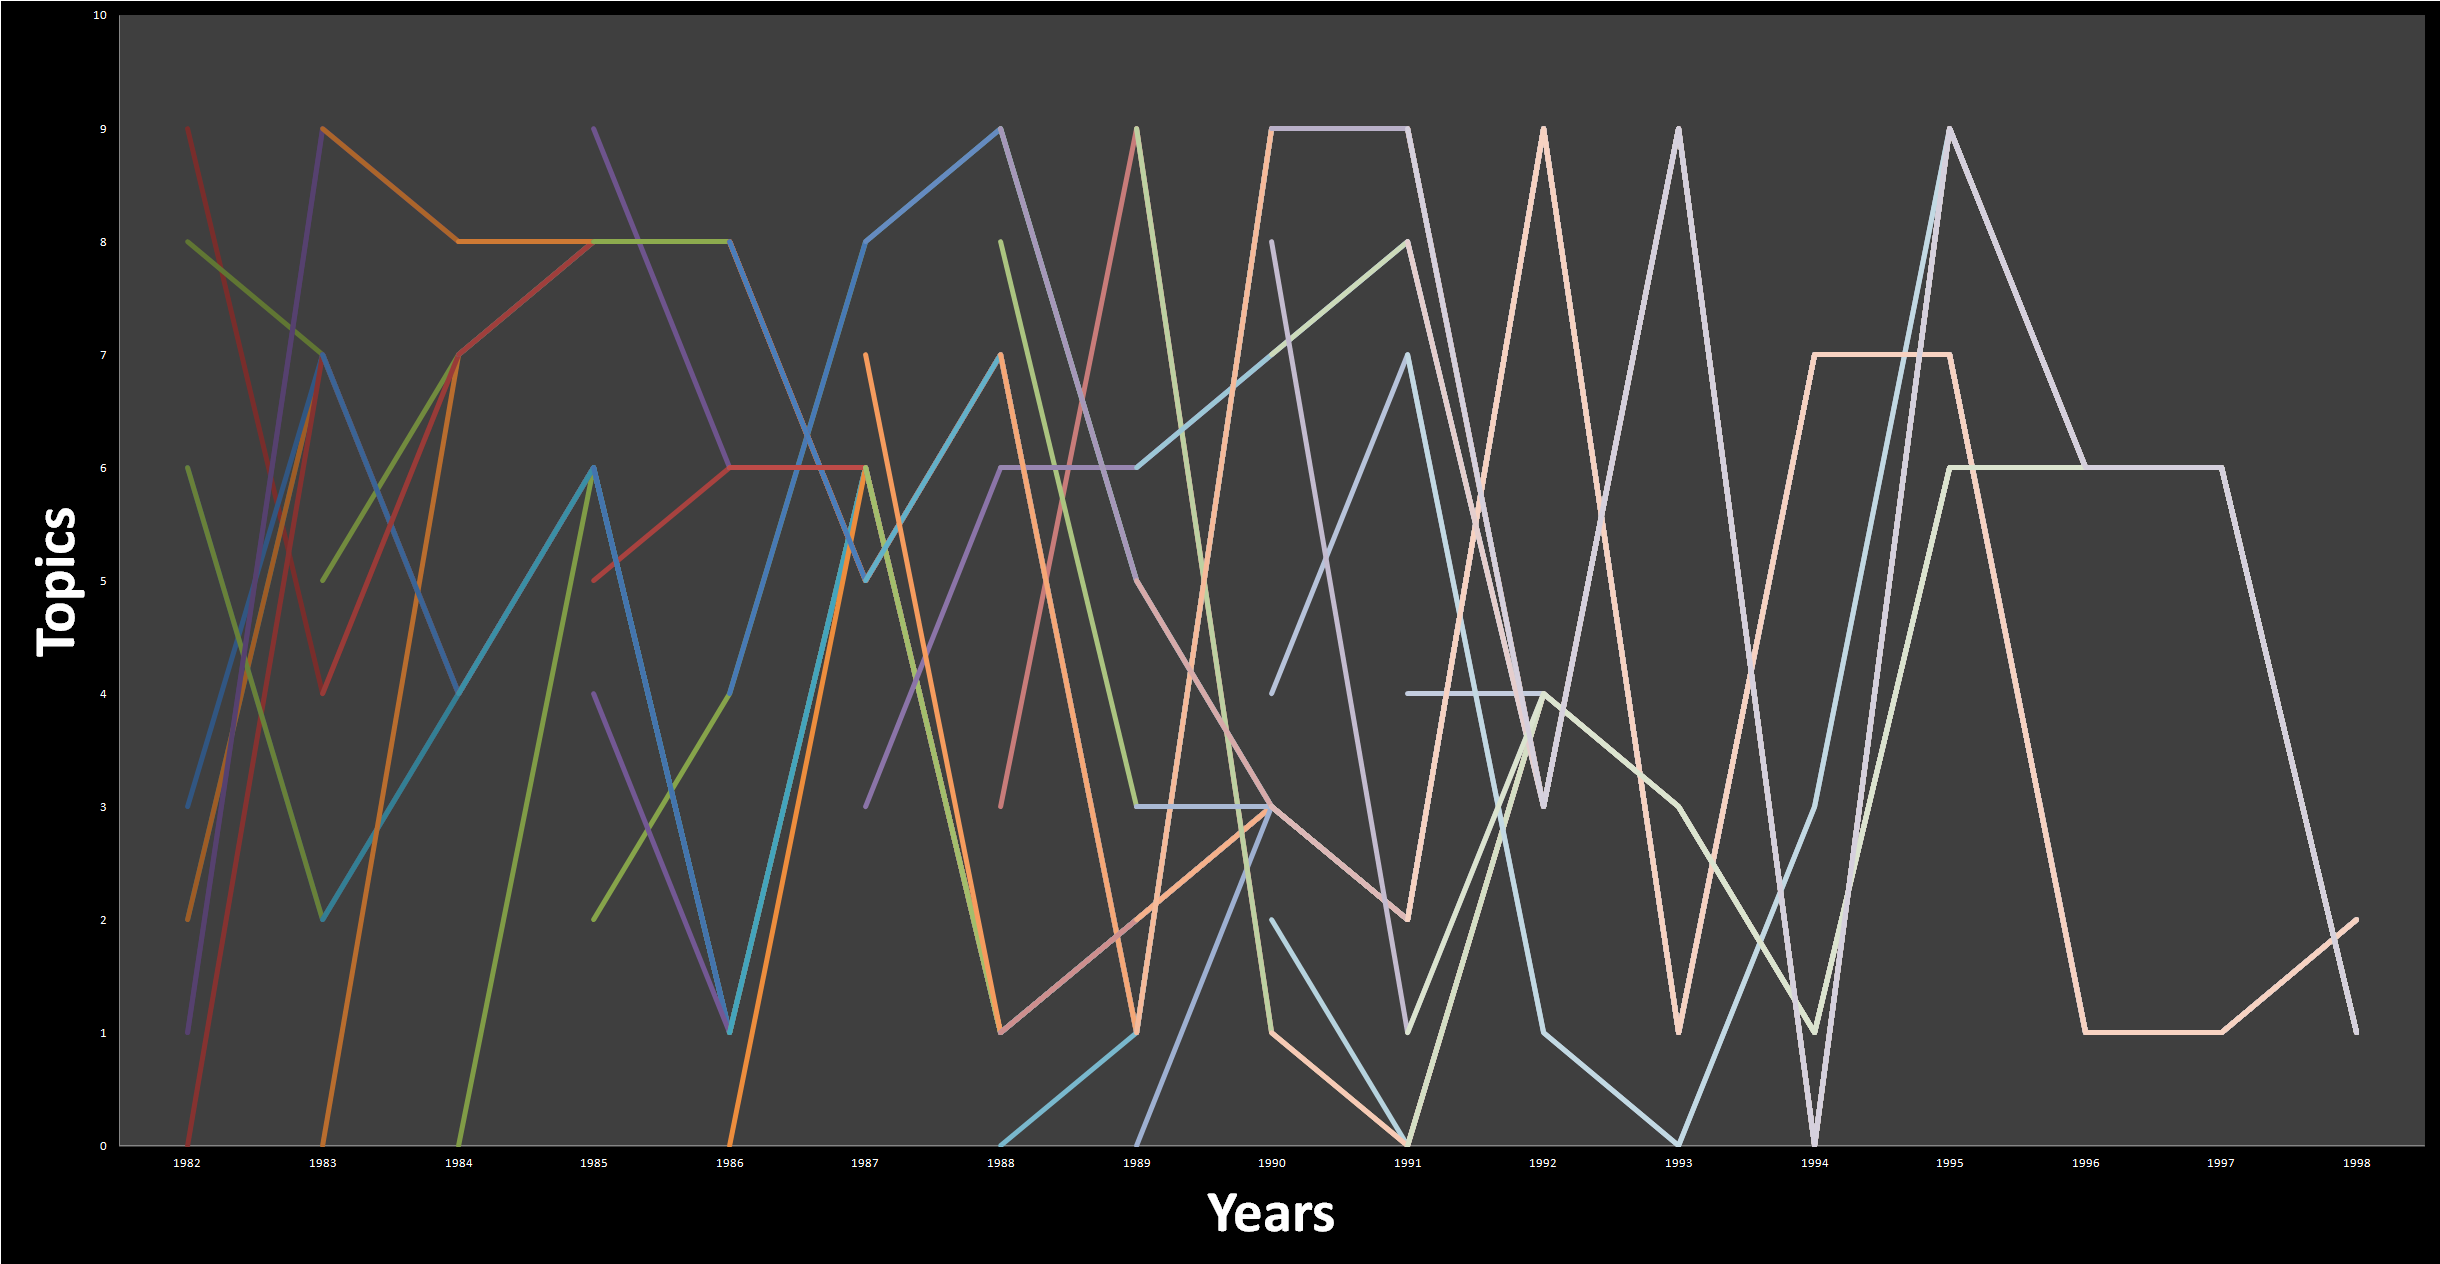
\includegraphics[width=1.3\textwidth, angle=270]{fig/tcg.png}
	\caption{An example of a Topic Convergence Graph for 10 years of data}
	\label{tcg}
\end{figure*}




% that's all folks
\end{document}


